% =====================================================================
%  Three Ways to Miss a Grasp
%  NextGen Scholars Research Paper Competition -- Original Research
%
%  Formatting follows paper_writing_framework.md: MLA 9, 12pt Times
%  New Roman, double spaced, 1in margins, "Talla N" page numbers,
%  sentence-case headings, tables captioned above, figures below.
%
%  BUILD:  pdflatex paper.tex   (run twice so references resolve)
%  Needs:  newtxtext, geometry, setspace, fancyhdr, graphicx, float,
%          caption, booktabs, pgfplots   -- all standard, all on Overleaf.
% =====================================================================

\documentclass[12pt,letterpaper]{article}

\usepackage[T1]{fontenc}
\usepackage[utf8]{inputenc}
\usepackage{newtxtext,newtxmath}   % Times New Roman metric-compatible
% If your TeX install lacks newtx, comment the line above and use:
%   \usepackage{mathptmx}
\usepackage[margin=1in]{geometry}
\usepackage{setspace}
\usepackage{fancyhdr}
\usepackage{graphicx}
\usepackage{float}
\usepackage{caption}
\usepackage{booktabs}
\usepackage{array}
\usepackage{pgfplots}
\pgfplotsset{compat=1.18}

\graphicspath{{figures/}{data/interim/comparison_sheets/}}

% ---- MLA page numbering: "Talla 4", upper right, no rule ----
\pagestyle{fancy}
\fancyhf{}
\rhead{Talla \thepage}
\renewcommand{\headrulewidth}{0pt}

% ---- Headings: 12pt, sentence case, no numbering ----
\makeatletter
\renewcommand{\section}{\@startsection{section}{1}{0pt}%
  {2.0ex plus 1ex minus .2ex}{1.0ex plus .2ex}{\normalsize\bfseries}}
\renewcommand{\subsection}{\@startsection{subsection}{2}{0pt}%
  {1.5ex plus 1ex minus .2ex}{0.6ex plus .2ex}{\normalsize\itshape}}
\makeatother

% ---- Captions: Table N. above, Fig. N. below ----
\captionsetup[table]{name=Table,labelsep=period,justification=raggedright,
                     singlelinecheck=false,font=normalsize,skip=4pt}
\captionsetup[figure]{name=Fig.,labelsep=period,justification=raggedright,
                      singlelinecheck=false,font=normalsize,skip=6pt}

% ---- MLA hanging indent for Works Cited (never tabs/spaces) ----
\newenvironment{workscited}{%
  \sloppy%
  \begin{list}{}{%
    \setlength{\leftmargin}{0.5in}%
    \setlength{\itemindent}{-0.5in}%
    \setlength{\labelwidth}{0pt}%
    \setlength{\labelsep}{0pt}%
    \setlength{\listparindent}{0pt}%
    \setlength{\topsep}{0pt}%
    \setlength{\partopsep}{0pt}%
    \setlength{\itemsep}{0pt}%
    \setlength{\parsep}{0pt}%
  }%
}{\end{list}}

\setlength{\parindent}{0.5in}

\begin{document}
\doublespacing

% ---------------------------------------------------------------
% MLA heading block, top left of page 1.
% ---------------------------------------------------------------
\begin{flushleft}
\setlength{\parindent}{0pt}
Anish Talla\\
NextGen Scholars Research Paper Competition\\
4 August 2026
\end{flushleft}

\begin{center}
Three Ways to Miss a Grasp: A Same-Metric Comparison of Rule-Based,
Learned, and Zero-Shot Vision-Language Prediction
\end{center}

% ===============================================================
\section*{Abstract}

A robot cannot pick anything up until something decides where on the
object to place the fingers and at what angle. That decision can come
from hand-written rules, from a model trained to predict grasps from
images, or from a general-purpose vision-language model never trained
on grasping at all. All three were built and scored against the same
external answer key, the Cornell Grasping Dataset's hand-labeled grasp
rectangles, on one held-out split of 123 images covering 35 objects
absent from training. Success was scored by the standard Cornell
rectangle metric, an angle within 30 degrees of a labeled grasp and an
intersection over union above 25\%. The learned system (fine-tuned
ResNet18) passed on 79.7\% of test images, the rule-based system on
57.7\%, and the zero-shot system (GPT-4o, one frozen prompt, averaged
over five runs per image) on 12.4\%. The rule-based figure is post-hoc
rather than held-out, since a defect found after the test set was
opened prompted a fix that raised it from 40.7\%, and both numbers are
reported throughout. The gap between the rule-based and learned systems
is significant under McNemar's exact test, and the vision-language
model trailed the rule-based system by 22.8 points even at its
best-of-five accuracy of 35.0\%, with an object-clustered 95\% interval
on that difference of [9.2, 35.6]. A secondary
analysis split test images by whether their labeled grasps run
diagonally. The three systems moved in three different directions,
though on only 20 diagonal images, so that finding is exploratory. The
model often named the correct part of the object while giving
coordinates that landed in none of the labeled grasp rectangles, on
53.4\% of calls against roughly 5\% for the other two systems. This
suggests GPT-4o may have more difficulty converting a visually
identified grasp region into usable coordinates than identifying one.
The study does not isolate that mechanism, so it is offered as a
hypothesis rather than a result.

% ===============================================================
\section*{Introduction}

Before a gripper closes on anything, something has to choose a contact
point, an approach angle, and how wide to open the fingers. Every piece
of motion that follows depends on that choice being roughly right. A
robot arm can be mechanically excellent and still fail constantly if
the thing telling it where to grip is wrong, which makes grasp
prediction one of the places where a small accuracy difference turns
into a large behavioral difference. It is also a problem that has to be
solved from thin information. In most real settings a robot gets a
camera image and little else, with no model of the object, no label
saying what it is, and no annotation marking the handle.

There are three broadly different ways to make that decision, and they
are not variations on a single method. A programmer can write the rule
directly, saying that mugs get grasped by the handle and bottles around
the neck. A model can be trained on thousands of hand-labeled examples
until it learns to map pixels to grasp rectangles. Or a general-purpose
vision-language model, trained on web text and images and never shown a
grasping dataset, can simply be asked in plain language where to grip.
Each is a bet about where the useful intelligence in a robot's
perception stack should live, whether in a person's explicit rules, in
weights fitted to task-specific data, or in a large model's general
knowledge of the world.

That third option is new enough that the field has not settled how to
use it. Foundation models arrived in robotics quickly, and the
literature is still working out which parts of a manipulation pipeline
they should own. The question matters practically, because the three
approaches demand very different resources. A lookup table needs only
hand-specified rules. A learned predictor needs a task-specific
annotated dataset and the compute to train on it. Prompting a hosted
vision-language model needs an API key and almost no setup, which is
exactly why it is tempting, and exactly why it deserves to be measured
rather than assumed.

Comparisons across those three families are rarer than you might
expect. Most published grasp-detection work benchmarks within a family,
comparing one trained architecture against another on the same dataset.
That produces useful leaderboards but does not tell you what you gain
or give up by changing approach entirely. Rule-based baselines, when
they appear, are often described rather than scored. Vision-language
models usually appear embedded inside a larger system, where their
individual contribution cannot be isolated. This project is a
comparison where all three sit on the same test images, produce the
same kind of output, and are scored by the same code.

The question is plain. Which approach actually works, and where does
each one break down? The second half matters at least as much as the
first. An accuracy number tells you a system is wrong. The shape of its
errors tells you why, and that is the part that transfers to whatever
somebody builds next.

The measuring apparatus is borrowed rather than invented, which matters
more than it might seem. A grasp here is a rectangle with a center
point, an orientation, and a width matched to how far the gripper
opens, the representation Jiang et al. introduced with the Cornell
Grasping Dataset (3304). Each image carries several labeled grasps
rather than one, since most objects can be picked up in more than one
valid way, and a prediction counts as correct if it matches any of
them. The matching rule is that the predicted angle falls within 30
degrees of a labeled grasp and the intersection over union between the
two rectangles exceeds 25\%, the convention established by Lenz et al.
(712). An external answer key was chosen deliberately. An earlier
design would have had me write the ground truth myself and then grade
my own rule-based system against it, which is close to circular. The
dataset's existing annotations remove that problem and make these
numbers comparable to published ones.

The three systems are as follows. System A is the rule-based baseline,
in which a COCO-pretrained detector identifies the object and a small
fixed table maps the detected category to a grasp region, with a
geometric fallback covering the images the detector cannot name. System
B is the learned predictor, a small convolutional network built from
scratch alongside fine-tuned ResNet18 and ResNet34 models, trained on
the Cornell training split. System C is GPT-4o, prompted directly with
the raw image and given no task-specific training whatsoever.

One thing this paper is not. It does not beat state-of-the-art grasp
detection and does not try to. Published pixel-wise systems reach
accuracies this work is not competing with. What this paper does is
measure, under conditions held as close to identical as the design
allows, how three families of technique fail, and argue that the shape
of each failure carries information the accuracy number does not.

What it does establish can be stated plainly. The three systems ran on
the same 123 held-out images through one shared scoring path. Their
ordering survives the change of sampling unit from image to object and
an object-clustered permutation test. The failure taxonomy then
separates the three families along lines that a single accuracy number
does not show.

% ===============================================================
\section*{Methods and discussion}

\subsection*{Dataset and evaluation}

The dataset used for evaluation is the Cornell Grasping Dataset,
roughly a thousand images of household objects, each with hand-labeled
grasp rectangles (Jiang et al.). A prediction counts as correct when
its angle falls within 30 degrees of some labeled grasp and its
rectangle intersection over union with that grasp exceeds 25\%, the
convention established by Lenz et al. Cornell's annotations are not
exhaustive, so passing this metric means matching a labeled grasp, not
that the grasp would physically succeed. The Jacquard dataset was
considered as an alternative, but its full distribution requires a
signed agreement and an approved non-free-email request. Object
identity was the hardest problem in building the split. No object may
appear in both training and test, or a model can memorize its grasp
rectangles from one split and be credited for recognizing the same
object in the other. Cornell provides no object-identity labels, so
identity had to be reconstructed from the image sequence. Comparing raw
pixel differences between consecutive frames failed, because the
dataset deliberately rotates each object between shots and same-object
and different-object scores overlapped. Instead, each frame was
segmented against the photography platform, and the resulting object
regions were compared to decide whether two frames showed the same
object or different ones.

Acceptance thresholds were set asymmetrically, since merging two
different objects into one group is less harmful than splitting one
real object into two. The ``different-object'' threshold was set below
the lowest score seen for any confirmed same-object pair, while the
``same-object'' threshold stayed loose. A 30-boundary stratified sample
was classified by both an AI assistant and a human, blind to each
other's calls. The AI's classifications matched the human's on 86.7\%
of its confident calls but only 40.0\% of the calls it flagged as
uncertain, so every uncertain call and every confident ``different'' call
was reviewed by hand. Confident ``same'' calls were accepted unreviewed,
since an error in that direction is harmless. The result is 234 objects
across 883 images, with 620 for training, 140 for validation, and 123
for test, as shown in Table~\ref{tab:split}. Published descriptions of
Cornell normally report around 240 objects, and the shortfall here is
expected rather than surprising, since the thresholds were deliberately
biased toward merging. Every merge that should have been a split lowers
the object count while keeping the merged group on one side of the
division, which is the error direction this design accepts on purpose.
Each object has at least one grasp rectangle, and most have several,
since most objects can be picked up more than one way.

\subsection*{System A, rule-based baseline}

System A is better described as a detector-assisted heuristic baseline
than a purely rule-based one. It detects the object with a
COCO-pretrained detector, which is itself a learned component, then
looks up the detected category in a fixed table of grasps. Nothing in
it is learned from grasp labels, which is the sense in which it is
rule-based. The table was committed before any evaluation code existed,
so no entry could be tuned toward a score. Since COCO's categories miss
more than half of what Cornell photographs, a geometric fallback that
does not rely on object recognition covers the objects the detector
misses, and that fallback handles the majority of test images.

One qualification belongs here rather than in Results. System A was
scored once at 40.7\% before the detector was found to be boxing
background clutter. The guard that fixed it was added after those test
predictions had been inspected, so although the recalibrated constant
used training data only, the decision to add the guard was prompted by
test behavior. That makes 57.7\% a post-hoc corrected figure rather
than a clean held-out one, and it weakens the comparisons that rest on
it, including the McNemar test against System B and the interval
comparison against System C. Both numbers are reported everywhere the
result appears.

A second limitation follows from the table's design. COCO's 80
categories do not cover most of what Cornell photographs, so many
objects have no table entry to begin with. And regardless of path,
System A's rectangle orientation is limited to 0 or 90 degrees, the
only two orientations the table and the box-based rule can express, so
any grasp that requires an angle in between is one System A cannot
produce.

\subsection*{System B, learned grasp predictor}

System B regresses a grasp rectangle directly from an image. A backbone
network extracts features, pools them, and a regression head predicts
the rectangle's parameters. Orientation is encoded as the sine and
cosine of twice the angle rather than a raw angle between 0 and 180
degrees. This accounts for the fact that a grasp rectangle rotated 180
degrees describes the same physical grasp. A raw-angle representation
would score that rotation as an entirely different grasp, while the
sine and cosine encoding treats it as identical. Redmon and Angelova
(1316) and Morrison et al. both used this same encoding.

System B trained three architectures on the same training split, a
small network built from scratch, a fine-tuned ResNet18, and a
fine-tuned ResNet34. The loss was computed against every labeled grasp
on an image, with only the best match backpropagated. Averaging toward
all of an image's grasps would pull a handle grasp and a rim grasp
toward a point on the object where neither is valid. Augmentation
applied the same affine transform to the grasp rectangle's corners as
to the image's pixels, rather than hand-writing a rule for how the
angle behaves under a flip.

System B's accuracy can look low next to two published Cornell results,
but neither is an even comparison. GR-ConvNet reports 97.7\% image-wise
and 96.6\% object-wise on an extended 1,035-image version of Cornell
(Kumra et al. 9626), and only the object-wise figure is on the same
footing as anything here. Redmon and Angelova report 84.9\%
object-wise (1316). GR-ConvNet is pixel-wise. It predicts a grasp at
every pixel in a single pass. System B does nothing of the kind. It
pools a backbone's features and regresses one rectangle for the whole
image, the same design Redmon and Angelova published, whose 84.9\%
object-wise score is the fairer target, as laid out in
Table~\ref{tab:redmon}. Every remaining gap points the same direction.
Redmon and Angelova used RGB-D and roughly 3,000 augmented examples per
image, while System B used RGB only and 620 real training images.

\subsection*{System C, zero-shot vision-language model}

System C prompts GPT-4o with each test image and asks where the two
gripper fingertips should touch, with no training or fine-tuning on
grasping. The prompt was developed on a batch of 30 training images and
frozen before test was opened.

The configuration was as follows. The model was called as
\texttt{openai/gpt-4o} through the OpenRouter API, at a 400-token cap,
with temperature left unset so the provider default applied and no seed
pinned, since run-to-run variation was one of the things being
measured. Images were sent at the dataset's native 640 by 480
resolution with no resizing, and the prompt told the model that
coordinates were in pixels of that image. Each repeat was an
independent single-turn completion with no prior messages, so the five
repeats of an image are five genuine draws rather than one
conversation. Transport failures were retried up to three times, but a
reply that arrived and then failed to parse was never retried, since
re-rolling malformed content would quietly convert a single-shot
baseline into a best-of-N one.

System C was not asked to output an angle. It returned two fingertip
points and a jaw width as JSON, and those three values determine all
four rectangle corners, which were then passed through the same frozen
function that produced every ground-truth angle in the dataset. No
rectangle parameter was supplied by me, and no radians-versus-degrees
convention had to be matched by hand. Each image was prompted five
times, and all five results are reported.

System C's 12.4\% does not mean vision-language models are bad at
spatial tasks. In several published grasping systems built on the same
kind of model, the model's output is a choice, a label, an order of
operations, or an image, and the pose of the gripper comes from
something else. FreeGrasp asks the model to decide which object to
grasp and in what order, using marks placed on the image (Jiao et al.).
Lan-grasp asks the model which part to grasp, then hands the pose to a
conventional planner (Mirjalili et al.). ThinkGrasp uses the model to
plan clutter removal (Qian et al.). Set-of-Mark asks the model to
select one of several labeled regions (Yang et al.). VLAD-Grasp asks
the model to draw the grasp using a virtual gripper (Kulshrestha et
al.).

In none of them does the model emit the pose coordinates itself, which
is exactly what System C is built to test. Does the gap come from the
coordinate-emission step, or from the model's inability to see the
object?

Of 615 calls, 365 failed on both angle and overlap simultaneously, far
more than either failure alone. A supplementary check asked whether
each predicted center fell inside the convex hull of an image's labeled
grasp rectangles, the loosest spatial test a prediction can fail.
System C failed it on 53.4\% of calls, against 7.0\% for System A and
6.5\% for System B. That gap is real, though the comparison isn't quite
even, since System B was trained on this distribution and System A's
center comes from a detected box or a segmentation, so both are close
to guaranteed to land on the object. System C is the only one free to
place a center anywhere. Reading the model's written explanations
alongside its coordinates on a sample of failures, the explanation
frequently named a real part of the object while the coordinates in the
same reply landed somewhere unrelated. That reading was informal rather
than a blinded coding study with a fixed rubric, so it should be
treated as the observation that motivated the hypothesis, not as a
measurement of how often the pattern holds.

Wang et al. document the same disconnect in an unrelated domain, with
models describing a correct solution to a visual puzzle in text, then
clicking hundreds of pixels away from it (Wang et al., sec. 5.3.2). The
tasks differ, but the failure, text and coordinates disagreeing within
one response, is the same.

\subsection*{The orientation axis}

Each system's design predicts something different about how orientation
should affect it. System A's representation cannot express a diagonal
grasp, System B's encoding handles rotation by construction, and System
C has no structural position on the question at all.

An image counts as axis-aligned when any one of its labeled grasps sits
within 15 degrees of 0 or 90 degrees, and as diagonal only when none
does. The rule is deliberately conservative, since a system that can
emit only axis-aligned rectangles still has a valid target whenever a
single labeled grasp is axis-aligned. It is also looser than the 30
degree scoring tolerance, so a diagonal image whose labeled grasps sit
20 degrees off axis is still reachable by an axis-aligned prediction.
That is why System A scores 40.0\% on the diagonal stratum rather than
near zero. Splitting the test set that way
produced exactly the predicted pattern. System A dropped 21.2 points on
the 20 diagonal images relative to axis-aligned ones, System B gained
12.3 points, and System C moved 2.0 points, as Fig.~\ref{fig:strata}
shows.

An axis-aligned box being unable to represent a diagonal grasp follows
from the representation alone, and a rotation-invariant encoding
handling rotation is the entire reason that encoding exists, so neither
point here is a discovery on its own. What I could not find precedent
for was using this split as a diagnostic. It checks whether each
system's accuracy rises or falls along an axis defined by the dataset's
own grasp-angle annotations, rather than reporting a single train and
test generalization number.

The diagonal stratum holds only 20 images, and the 95\% intervals
around System B's and System C's per-stratum accuracies are wide enough
that their point changes there are not reliably distinguishable from
noise. Only System A's drop was predicted from its representation
before the stratum was scored, which makes it pre-registered rather
than found afterward. Pre-registering a direction is not the same as
confirming an effect, and no interaction test between system and
stratum was run, so this remains exploratory too. System C's near-flat
response is at least consistent with the coordinate-binding hypothesis
explored later, since a system with no working orientation signal
should look flat on this split, and it does.

A second split, by the number of grasps labeled per image, was tested
as a difficulty proxy. More labeled grasps should mean more chances for
a prediction to match. It did not behave that way. All three systems
did worst on the images with the most labeled grasps. The likely
explanation is that annotators labeled more grasps on objects that
afford more of them, so the count tracks object complexity rather than
how generous the metric is.

\subsection*{What this means}

This explanation makes a testable prediction. Removing System C's
ability to output coordinates directly should help if the problem is
binding reasoning to those coordinates rather than perceiving the
object, and should make no difference if the problem is perception. Two
published results are consistent with the first case, though neither
was designed as a test of it. Set-of-Mark lets zero-shot GPT-4V beat a
fine-tuned specialist on RefCOCOg purely by replacing coordinate output
with region selection (Yang et al.). VLAD-Grasp scores far above System
C on this same dataset, training-free, by having the model draw the
grasp instead of stating it (Kulshrestha et al.).

VLAD-Grasp is the comparison that most complicates System C's result,
but two things keep it from being a number that can be set directly
against 12.4\%. It does not simply ask for a picture instead of a
coordinate. It then predicts depth, segments the object, and aligns 3D
point clouds to recover a pose, a pipeline System C has no equivalent
to. It also counts a grasp correct on overlap alone, with no angle
requirement, and reports 91.4\% under that looser test on a set of 70
unseen Cornell objects. That the same evaluation scores GR-ConvNet at
72.1\%, against the 97.7\% GR-ConvNet reports for itself, shows the two
protocols are not directly comparable. The dropped angle criterion is
what matters here, since orientation is the variable this paper's
results depend on most. It is also a different model rather than the
same one, since the current revision of that paper names GPT-5 as its
primary model, so it evidences what a vision-language model can do
without emitting coordinates, not what GPT-4o specifically can do.

Even with that caveat, two zero-shot uses of a pretrained
vision-language model on the same benchmark produce very different
outcomes, and the one that works never asks for a coordinate.
Requesting raw coordinates appears to carry a cost unrelated to whether
the model can see the object.

The sine and cosine encoding dates to 2015, learned models have beaten
rule-based baselines on Cornell for a decade, and imprecise
vision-language coordinates are already documented elsewhere, so none
of this is new by itself. Putting a number on that last weakness, on a
standard benchmark against two baselines, with an account of the
mechanism behind it, is what this experiment adds.

A one-million-parameter network built from scratch never learned the
task by any reasonable standard, reaching 23.6\% after a learning-rate
sweep confirmed that wasn't a tuning artifact. It still beat GPT-4o
(System C) by 11 points, which I did not expect.

Three bugs in my own code were caught before any result was reported,
each of which would have produced a plausible but wrong number. All
three turned up the same way. An automated result didn't match an
independent calculation, and neither was trusted until the disagreement
was explained.

% ===============================================================
\section*{Limitations}

This test was limited to using a single split of the dataset relative
to the five-fold cross-validation that is used by most published
results using the Cornell dataset. Seven of the 35 object groups in the
test split contain only a single image of the object, so the results for
those objects are not as precise as they could be. Jacquard, considered
as a second dataset source, was unavailable during this study, so no
results were performed to test the generalization of these techniques
across datasets. An early formatting check on roughly 550 grasp
rectangles likely touched a small number of images that later landed in
the test split. No threshold, constant, or lookup entry was derived
from that check, but it should be disclosed.

The three systems did not receive comparable engineering effort, which
cuts against reading this as a controlled comparison. System B got three
architectures, a five-point learning-rate sweep, a tuned loss weight,
and validation-based model selection. System C got one prompt, frozen
after development on 30 training images and never revised. Freezing it
protected test-set integrity and I would do it again, but prompt design
is the vision-language equivalent of architecture search, and I ran
architecture search for one system and not the other. So 12.4\%
measures what one un-iterated prompt achieves, not a ceiling for
zero-shot GPT-4o. The gap to System B is wide enough that prompt
iteration is unlikely to reverse the ordering, but the specific number
should not be quoted as the model's best.

System C's potential contamination by the dataset was examined. While
the dataset is a publicly available dataset that is mirrored by many
organizations, a test of ten images of objects of various categories
asked the language model to identify the source of the images returned
no recognitions. This is a weak indicator of contamination of the model
by the dataset, but contamination of the language model would only have
led to an increase in System C's score, which is already the lowest of
the three systems. So the failure of System C in comparison to the
other models holds even in the worst-case scenario of contamination of
the model by the dataset.

Every interval and significance test reported here treats its unit of
analysis as independent, and none of them are. System C's interval is
computed over 615 calls, but those are five repeats of 123 images, not
615 independent trials, so it is narrower than the data support. The
image-level intervals and McNemar tests for Systems A and B have the
same problem one level up, since the 123 test images are grouped within
35 objects and images of one object are not independent of each other.
The stated population is unseen objects, so the correct sampling unit
is the object. The object-clustered intervals and differences reported
in the results section are the primary ones, and every Wilson interval
quoted per system is image-level and narrower than the data support.
Weighting each object equally rather than by how many images it
contributes lowers every system, System A to 51.3\%, System B to
75.4\%, and System C to 10.5\%, because test object groups range from
one image to nine. The ordering is unchanged.

The findings of the results relative to the orientation of the objects
was based on a sample size of only 20 objects. Additionally, the other
findings of this test were made of one model, one method of posing the
question to that model, and the one aspect of the task of grasping that
is examined, the coordinates of the grasp, so these results describe
that one setup rather than vision-language models generally.

All of the inputs to the models used in this test were images in RGB
format only. No depth information from the objects was used as an input
to any of the tested models.

% ===============================================================
\section*{Results}

\subsection*{The data split}

\begin{table}[H]
\centering
\caption{Object-wise split of the Cornell Grasping Dataset. No object
appears in more than one split.}
\label{tab:split}
\begin{tabular}{lrr}
\toprule
Split & Objects & Images \\
\midrule
Train      & 164 & 620 \\
Validation &  35 & 140 \\
Test       &  35 & 123 \\
\midrule
Total      & 234 & 883 \\
\bottomrule
\end{tabular}
\end{table}

The split covers 234 objects across 883 images, divided roughly 70/15/15
by object count. No object appears in more than one split.

Of the 884 frame boundaries examined, 251 (28.4\%) fell into the
ambiguous band. 139 of those were decided by hand, and the remaining
112 were confident same-object calls accepted without review. Six
stayed genuinely uncertain after full review. Four carried a lean
toward ``same object'' and were resolved that way, and the other two had
no lean. One image from the smaller side of each was dropped instead,
accounting for the 883 images retained out of 885.

\begin{figure}[H]
\centering
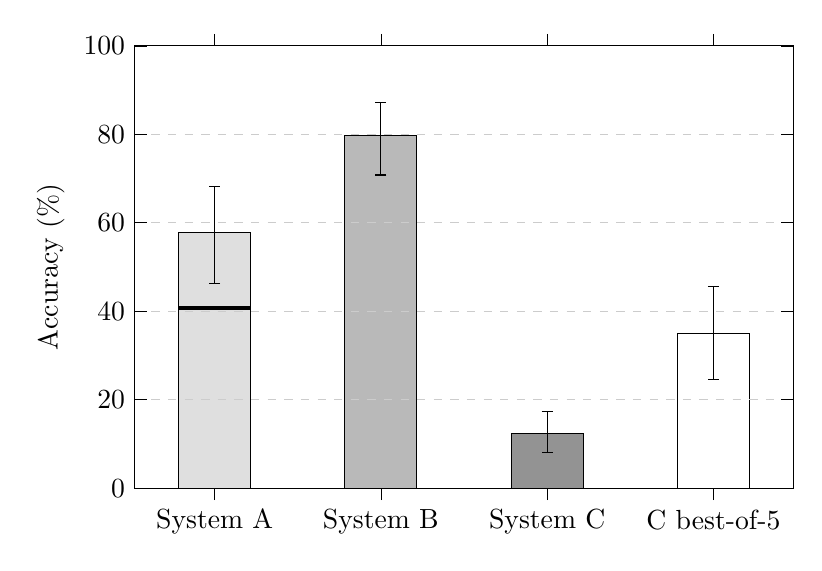
\begin{tikzpicture}
\begin{axis}[
  width=0.82\textwidth, height=7.2cm,
  ybar,
  bar width=26pt,
  ymin=0, ymax=100,
  ylabel={Accuracy (\%)},
  ylabel style={font=\normalsize},
  symbolic x coords={A,B,C,Cb},
  xtick={A,B,C,Cb},
  xticklabels={{System A},{System B},{System C},{C best-of-5}},
  xticklabel style={font=\normalsize},
  yticklabel style={font=\normalsize},
  enlarge x limits=0.16,
  ymajorgrids=true,
  grid style={dashed,gray!40},
  axis on top,
  tick style={black},
]
% each bar placed at its own symbolic x, so shift is suppressed
\addplot[fill=gray!25,draw=black,bar shift=0pt,
  error bars/.cd, y dir=both, y explicit]
  coordinates { (A, 57.7) += (0,10.5) -= (0,11.5) };
\addplot[fill=gray!55,draw=black,bar shift=0pt,
  error bars/.cd, y dir=both, y explicit]
  coordinates { (B, 79.7) += (0,7.4)  -= (0,8.9)  };
\addplot[fill=gray!85,draw=black,bar shift=0pt,
  error bars/.cd, y dir=both, y explicit]
  coordinates { (C, 12.4) += (0,5.0)  -= (0,4.4)  };
\addplot[fill=white,draw=black,bar shift=0pt,
  error bars/.cd, y dir=both, y explicit]
  coordinates { (Cb, 35.0) += (0,10.5) -= (0,10.4) };
% System A before the post-hoc guard was added
\addplot[only marks,mark=-,mark size=13pt,very thick,draw=black]
  coordinates { (A, 40.7) };
\end{axis}
\end{tikzpicture}
\caption{Test-set accuracy with 95\% object-clustered intervals, the
primary intervals in this paper. System A 57.7 [46.2, 68.2], System B
79.7 [70.8, 87.1], System C 12.4 [8.0, 17.4], and System C's
best-of-five ceiling 35.0 [24.6, 45.5], which requires five calls per
image rather than one. The horizontal rule across the System A bar
marks 40.7\%, the figure that system scored before the post-hoc
geometric guard was added, so the size of that correction is visible
here rather than only in the text.}
\label{fig:headline}
\end{figure}

The ordering in Fig.~\ref{fig:headline} is the paper's main result, and
the per-system subsections below give the counts behind each bar.

\subsection*{System A}

System A achieved 57.7\% on the test split (71 of 123), with a 95\%
Wilson interval of [48.9, 66.1]. Of the 52 failed predictions, 13
missed the orientation step alone.

The two paths performed differently. The detector fired on 39.8\% of
test images (49 of 123). Counting every image where it fired on nothing
as a failure gives 22.8\% (28 of 123), while accuracy on the images
where it did fire was 57.1\% (28 of 49). The fallback geometric system
attempted 66 images and found no grasp on 8. Accuracy by object
category was uneven, with all apples correct (6 of 6) but only 8 of 11
cell phones, none of the cups or bowls, and none of the laptops.

The table was evaluated once at 40.7\% before the detector was found to
be boxing background clutter. A geometric guard requiring the box to
contain the object's centroid, plus one constant recalibrated on
training, raised the result to 57.7\%. Both figures stay on record. The
detector-only number moved only from 22.0\% to 22.8\%.

\subsection*{System B}

System B is compared with its closest published counterpart in
Table~\ref{tab:redmon}.

\begin{table}[H]
\centering
\caption{System B compared with Redmon and Angelova's Direct
Regression, the closest published architecture.}
\label{tab:redmon}
\begin{tabular}{lll}
\toprule
 & Redmon and Angelova (2015) & System B (ResNet18) \\
\midrule
Architecture         & Global regression & Global regression \\
Orientation encoding & sin/cos of twice the angle
                     & sin/cos of twice the angle \\
Input                & RGB-D & RGB only \\
Training data        & \textasciitilde{}3,000 augmented per image
                     & 620 real images \\
Object-wise accuracy & 84.9\% & 79.7\% \\
\bottomrule
\end{tabular}
\end{table}

It achieved 79.7\% on the test split (98 of 123), with a 95\% Wilson
interval of [71.7, 85.8]. Its mean angle error of 3.9 degrees is
measured only on the predictions it got right, against whichever
labeled grasp the metric matched, so it describes how precisely System
B orients a grasp when it succeeds and says nothing about the 25 it
missed. System B's ResNet34 model achieved 70.7\% (87 of 123) with an
average intersection over union of 0.424 of its grasps with the labeled
grasps. The from-scratch model achieved 23.6\% (29 of 123) with an
average angle error of 24.2 degrees. Parameter counts were 11.3M,
21.4M, and 1.0M respectively.

System B's ResNet18 outperformed ResNet34 on validation as well as test
(83.6\% versus 77.1\%), so the selection held across both splits. The
validation-to-test gap (3.9 points) sits well inside the 6.7 to 11.9
point swings seen between epochs during training, so it isn't evidence
of overfitting. The from-scratch network got its own five-point
learning-rate sweep on validation, scoring 21.4\% at 3e-5, 27.1\% at
1e-4, 26.4\% at 3e-4, 20.0\% at 1e-3, and 22.9\% at 3e-3. The rate of
1e-4 was selected.

System B's ResNet18 model missed 25 of 123 test images. Of those missed
images, 4 failed on determining the angle of the object to grasp, while
15 failed on the overlap of the bounding box around the object with any
labeled grasp in the image. ResNet34 failed to detect grasps in 36
images, while the from-scratch model missed 94 images. One of those
angle-only failures is shown in Fig.~\ref{fig:anglefail}.

\begin{figure}[H]
\centering
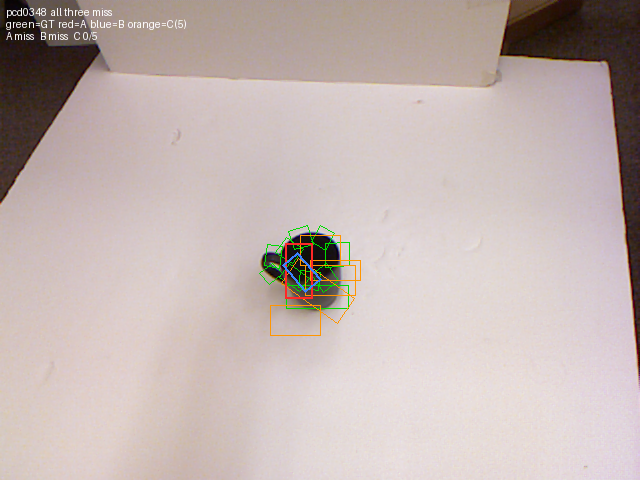
\includegraphics[width=0.8\textwidth]{compare_0348.png}
\caption{An orientation-only failure. The predicted grasping rectangle
correctly overlaps the object (intersection over union of 0.38) but
rotates 47 degrees from any labeled grasp. Of the four ResNet18
angle-only failures (pcd0676, pcd0348, pcd0824, pcd0316), only pcd0348
has a rendered sheet, which is why it was chosen.}
\label{fig:anglefail}
\end{figure}

\subsection*{System C}

System C achieved 12.4\% accuracy on test images (76 of 615 calls),
with a 95\% Wilson interval of [10.0, 15.2]. Each of the five
independent runs achieved 13.0\%, 14.6\%, 13.8\%, 10.6\%, and 9.8\%
accuracy. The best-of-five attempts achieved 35.0\% (43 of 123). A
consensus rule that scores whichever single repeat agrees most closely
with the other four, since continuous rectangles cannot be
majority-voted directly, reached 12.2\%. Neither of these is the
headline figure. Both require either multiple calls per image or
knowing the answer in advance. The model returned a parseable reply on
614 of 615 calls (99.8\%), and every non-parsing call counts as a miss
in the headline figure.

\begin{table}[H]
\centering
\caption{Which criterion each prediction missed, computed through one
shared scoring path for all three systems.}
\label{tab:taxonomy}
\begin{tabular}{lrrr}
\toprule
Outcome & System A (of 123) & System B (of 123) & System C (of 615) \\
\midrule
Correct       & 71 (57.7\%) & 98 (79.7\%) & 76 (12.4\%) \\
Angle only    & 13 (10.6\%) &  4 (3.3\%)  & 85 (13.8\%) \\
Overlap only  & 18 (14.6\%) & 15 (12.2\%) & 88 (14.3\%) \\
Both          & 13 (10.6\%) &  6 (4.9\%)  & 365 (59.3\%) \\
No prediction &  8 (6.5\%)  &  0 (0.0\%)  & 1 (0.2\%) \\
\bottomrule
\end{tabular}
\end{table}

The failure taxonomy in Table~\ref{tab:taxonomy} shows where the three
systems differ most. For the geometric check described in Methods,
System C's predicted center fell outside the convex hull containing
every labeled grasp on 53.4\% of calls (328 of 614). System A showed
failures of this type on 7.0\% of the calls in which it attempted a
grasp (8 of 115 scored calls), and System B on 6.5\% (8 of 123).
Table~\ref{tab:hull} puts the three side by side.

\begin{table}[H]
\centering
\caption{Predicted grasp centers falling outside the convex hull of an
image's labeled grasps. This is a diagnostic across scored calls, not a
partition, so it overlaps the failure categories in
Table~\ref{tab:taxonomy} rather than adding to them.}
\label{tab:hull}
\begin{tabular}{lrr}
\toprule
System & Calls scored & Center outside hull \\
\midrule
System A &  115 &   8 (7.0\%)  \\
System B &  123 &   8 (6.5\%)  \\
System C &  614 & 328 (53.4\%) \\
\bottomrule
\end{tabular}
\end{table}

Agreement across System C's five runs was low. Mean self-agreement was
22.0\%, with a mean pairwise angle spread of 5.8 degrees and mean
pairwise intersection over union of 0.13. The distribution of how many
of five repeats scored correct per image appears in
Fig.~\ref{fig:repeats}. That puts 81 of 123 images (65.9\%) at a fully
consistent outcome, leaving 42 where the same model on the same pixels
sometimes passed and sometimes didn't.

\begin{figure}[H]
\centering
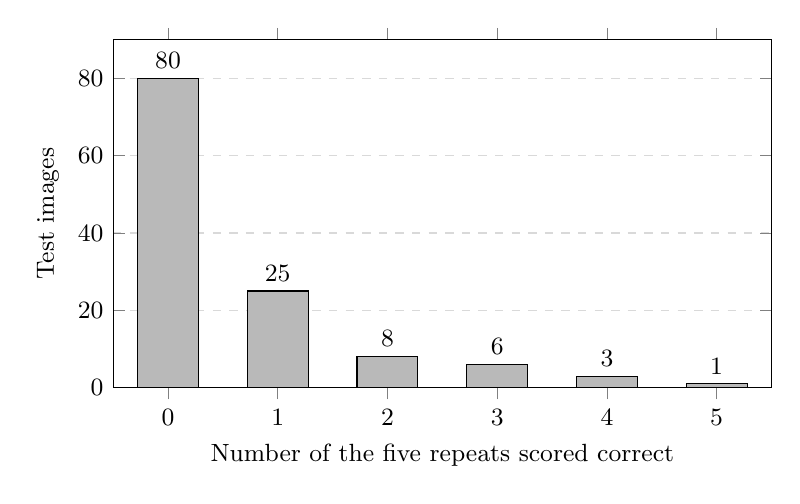
\begin{tikzpicture}
\begin{axis}[
  width=0.82\textwidth, height=6.0cm,
  ybar, bar width=22pt,
  ymin=0, ymax=90,
  xlabel={Number of the five repeats scored correct},
  ylabel={Test images},
  xtick={0,1,2,3,4,5},
  ymajorgrids=true, grid style={dashed,gray!30},
  nodes near coords, every node near coord/.append style={font=\small},
  tick label style={font=\small}, label style={font=\small},
]
\addplot[fill=gray!55,draw=black]
  coordinates {(0,80) (1,25) (2,8) (3,6) (4,3) (5,1)};
\end{axis}
\end{tikzpicture}
\caption{System C repeat consistency across 123 test images. On 80
images no repeat succeeded and on only one image did all five, leaving
42 images where the same model on the same pixels sometimes passed and
sometimes did not.}
\label{fig:repeats}
\end{figure}

Self-agreement carries usable signal. Restricting to the 21.1\% of
images where at least 40\% of repeat pairs agreed lifts best-of-five
accuracy to 57.7\% on those images, against 35.0\% at full coverage.
The match with System A's single-prediction 57.7\% is a coincidence.
This describes
which of several repeated calls to trust, not a fourth accuracy figure
to set against Systems A and B.

\subsection*{Cross-system comparison}

System A against System B is significant under McNemar's exact test
(p = 1.4e-4), the 38-versus-11 split described below. System C was
tested separately against each of its five runs rather than pooled, and
the least significant of the five is reported, p = 5e-12 against System
A and p = 1.6e-20 against System B.

Every interval quoted so far treats images, or in System C's case
individual calls, as independent. They are not, because the 123 test
images sit inside 35 objects. Resampling whole objects with replacement
widens all of them. System A becomes [46.2, 68.2], System B
[70.8, 87.1], System C [8.0, 17.4], and System C's best-of-five
[24.6, 45.5]. Checking whether two such intervals overlap is a weak
test, so the differences were bootstrapped directly on the same
resamples. System B leads System A by 22.0 points [9.7, 35.1], System A
leads System C's best-of-five by 22.8 points [9.2, 35.6], and System A
leads System C at one call per image by 45.4 points [33.8, 55.6]. None
of those intervals contains zero, and an object-clustered permutation
test agrees at p = 0.003, 0.006, and 5e-5. The ordering of the three
systems survives the change of sampling unit. The Wilson intervals
reported per system above are image-level and should be read as the
narrower of the two.

\begin{figure}[H]
\centering
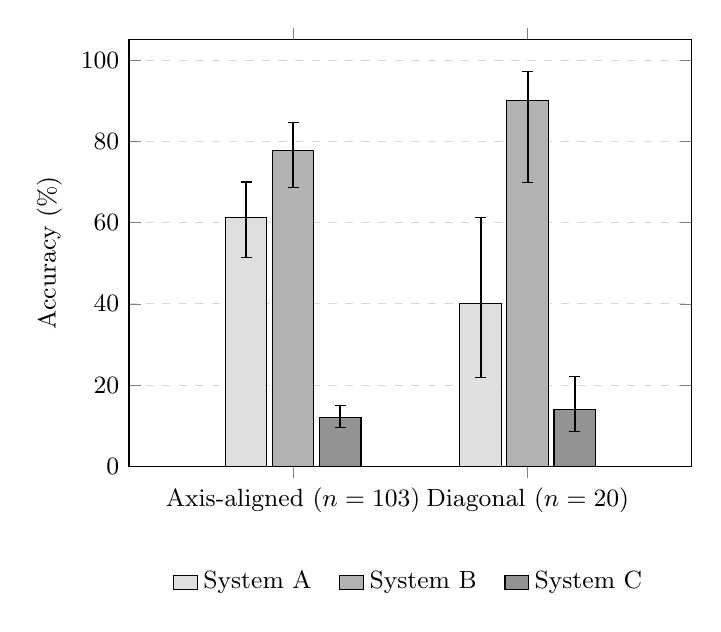
\begin{tikzpicture}
\begin{axis}[
  width=0.72\textwidth, height=7.0cm,
  ybar, bar width=15pt,
  ymin=0, ymax=105,
  symbolic x coords={axisaligned,diagonal},
  xtick=data,
  xticklabels={Axis-aligned ($n=103$), Diagonal ($n=20$)},
  enlarge x limits=0.7,
  ylabel={Accuracy (\%)},
  ymajorgrids=true, grid style={dashed,gray!30},
  legend style={at={(0.5,-0.22)}, anchor=north, legend columns=3,
                draw=none, font=\small, /tikz/every even column/.append style={column sep=8pt}},
  legend image code/.code={\draw[#1,draw=black]
     (0cm,-0.09cm) rectangle (0.30cm,0.09cm);},
  tick label style={font=\small}, label style={font=\small},
  error bars/error bar style={black,thick},
]
\addplot[fill=gray!25,draw=black,
  error bars/.cd, y dir=both, y explicit]
  coordinates {
    (axisaligned, 61.2) += (0,8.8)  -= (0,9.7)
    (diagonal,    40.0) += (0,21.3) -= (0,18.1)
  };
\addplot[fill=gray!60,draw=black,
  error bars/.cd, y dir=both, y explicit]
  coordinates {
    (axisaligned, 77.7) += (0,6.9)  -= (0,9.0)
    (diagonal,    90.0) += (0,7.2)  -= (0,20.1)
  };
\addplot[fill=gray!85,draw=black,
  error bars/.cd, y dir=both, y explicit]
  coordinates {
    (axisaligned, 12.0) += (0,3.1)  -= (0,2.5)
    (diagonal,    14.0) += (0,8.1)  -= (0,5.5)
  };
\legend{System A, System B, System C}
\end{axis}
\end{tikzpicture}
\caption{Accuracy by orientation stratum with 95\% Wilson intervals.
Axis-aligned, 103 images: System A 61.2 [51.5, 70.0], System B 77.7
[68.7, 84.6], System C 12.0 [9.5, 15.1]. Diagonal, 20 images: System A
40.0 [21.9, 61.3], System B 90.0 [69.9, 97.2], System C 14.0
[8.5, 22.1]. These are image-level rather than object-clustered, so
they are the narrower reading. The three systems move in three
directions, but the diagonal intervals are already wide enough that
only System A's drop, which was predicted from its representation
beforehand, should carry weight.}
\label{fig:strata}
\end{figure}

Systems A and B agreed on 74 of 123 images, both correct on 60 and both
wrong on 14. Of the 49 they disagreed on, System B alone was correct on
38 and System A alone on 11. Counting System C as correct whenever any
of its five repeats passed, all three systems succeeded together on 22
images and failed together on 10. Fig.~\ref{fig:threeway} shows one
such image with all three systems overlaid.

All three systems did worst on the images with the most labeled grasps
(8 to 25), rather than the fewest, the opposite of what a
more-labels-means-easier-match hypothesis would predict. In that group,
System A scored 48.0\%, System B 64.0\%, and System C 11.2\%.

\begin{figure}[H]
\centering
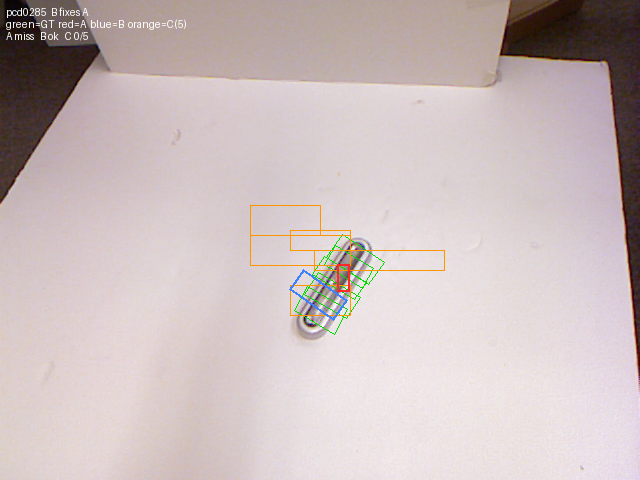
\includegraphics[width=0.8\textwidth]{compare_0285.png}
\caption{All three systems on one image. Labeled ground-truth grasps
are green, System A red, System B blue, and System C's five repeats
orange.}
\label{fig:threeway}
\end{figure}

% ===============================================================
\section*{Conclusion}

System A's accuracy of 57.7\% is lower than System B's 79.7\%, and
higher than System C's 12.4\% for zero-shot GPT-4o.

System A places a rectangle on the object often enough to score, though
its detector fires on only 49 of 123 images and a geometric fallback
carries the rest, and it cannot rotate the gripper at all, since an
axis-aligned box has no way to express a diagonal grasp. System B
rotates well, to within about four degrees on the predictions it gets
right, with most of its remaining error coming from placement rather
than orientation. System C produced the most distinctive error pattern
in this comparison. Its coordinates are frequently not bound to the
object its own text has just described correctly, so it fails before
either of the other two questions is even reached.

The third failure matters most because another system does not have it.
VLAD-Grasp runs a vision-language model zero-shot on this same dataset
and scores far higher, though it uses a different model, adds a
geometry pipeline System C has no equivalent to, and grades itself
without the angle criterion used here, so the two numbers cannot be
compared directly. The same text-coordinate divergence has turned up
independently in a different task with the same kind of model, which is
at least some evidence it is a property of the model rather than an
artifact of this one prompt.

Rerunning System C with Set-of-Mark prompting, having it select among
labeled regions instead of emitting coordinates, would test this
directly. If the error persists anyway, the problem is perception, not
coordinate binding, and that would be worth knowing too. This
experiment has not yet been run.

% ===============================================================
\newpage
\begin{center}
Works Cited
\end{center}

\begin{workscited}

\item Jiang, Yun, et al. ``Efficient Grasping from RGBD Images: Learning
Using a New Rectangle Representation.'' \textit{2011 IEEE International
Conference on Robotics and Automation (ICRA)}, IEEE, 2011, pp. 3304-11.

\item Jiao, Runyu, et al. ``Free-Form Language-Based Robotic Reasoning
and Grasping.'' \textit{arXiv}, 17 Mar. 2025, arxiv.org/abs/2503.13082.

\item Kulshrestha, Manav, et al. ``VLAD-Grasp: Zero-Shot Grasp Detection
via Vision-Language Models.'' \textit{arXiv}, 8 Nov. 2025,
arxiv.org/abs/2511.05791.

\item Kumra, Sulabh, et al. ``Antipodal Robotic Grasping Using
Generative Residual Convolutional Neural Network.'' \textit{2020
IEEE/RSJ International Conference on Intelligent Robots and Systems
(IROS)}, IEEE, 2020, pp. 9626-33.

\item Lenz, Ian, et al. ``Deep Learning for Detecting Robotic Grasps.''
\textit{The International Journal of Robotics Research}, vol. 34, no.
4-5, 2015, pp. 705-24.

\item Mirjalili, Reihaneh, et al. ``Lan-grasp: Using Large Language
Models for Semantic Object Grasping and Placement.'' \textit{arXiv}, 8
Oct. 2023, arxiv.org/abs/2310.05239.

\item Morrison, Douglas, et al. ``Closing the Loop for Robotic Grasping:
A Real-Time, Generative Grasp Synthesis Approach.'' \textit{Robotics:
Science and Systems XIV}, 2018.

\item Qian, Yaoyao, et al. ``ThinkGrasp: A Vision-Language System for
Strategic Part Grasping in Clutter.'' \textit{arXiv}, 16 July 2024,
arxiv.org/abs/2407.11298.

\item Redmon, Joseph, and Anelia Angelova. ``Real-Time Grasp Detection
Using Convolutional Neural Networks.'' \textit{2015 IEEE International
Conference on Robotics and Automation (ICRA)}, IEEE, 2015, pp. 1316-22.

\item Wang, Junyu, et al. ``COGNITION: From Evaluation to Defense
against Multimodal LLM CAPTCHA Solvers.'' \textit{arXiv}, 2 Dec. 2025,
arxiv.org/abs/2512.02318.

\item Yang, Jianwei, et al. ``Set-of-Mark Prompting Unleashes
Extraordinary Visual Grounding in GPT-4V.'' \textit{arXiv}, 17 Oct.
2023, arxiv.org/abs/2310.11441.

\end{workscited}

\end{document}
